\chapter{Algoritmo Pollard-Rho}
Em 1978, Pollard veio com um método ``Monte-Carlo'' para resolver o problema do logaritmo discreto. Desde então, o método foi modificado para resolver o ECDLP. Como o algoritmo Pollard-Rho é atualmente o algoritmo mais rápido para resolver o ECDLP, então a segurança do ECC depende da eficiência desse algoritmo. Teoricamente, se o algoritmo Pollard-Rho é capaz de resolver o ECDLP eficientemente e em um tempo relativamente curto, então o sistema estará inseguro. \cite{Mandy:2007}

A estratégia do algoritmo é produzir uma sequência de termos gerados randomicamente $(R_i, a_i, b_i)$, onde \(R_i\) é um ponto na curva \(E\) e \(a_i\)  \(b_i\) estão em $\mathbb{F}_p$ sobre a qual a curva elíptica \(E\) está definida. Desde que $E(\mathbb{F}_p)$ seja um grupo finito, a sequência eventualmente irá torna-se periódica e voltará para um termo anterior da sequência. Usa-se essa periodicidade para resolver ECDLP. Como nem sempre a sequência volta para o primeiro termo, um diagrama da sequência parecerá com a letra Grega \(\rho\) (Ver figura \ref{fig:rho}). Por este motivo esse método é chamado de Pollard-Rho.

\begin{figure}[h]
\centering
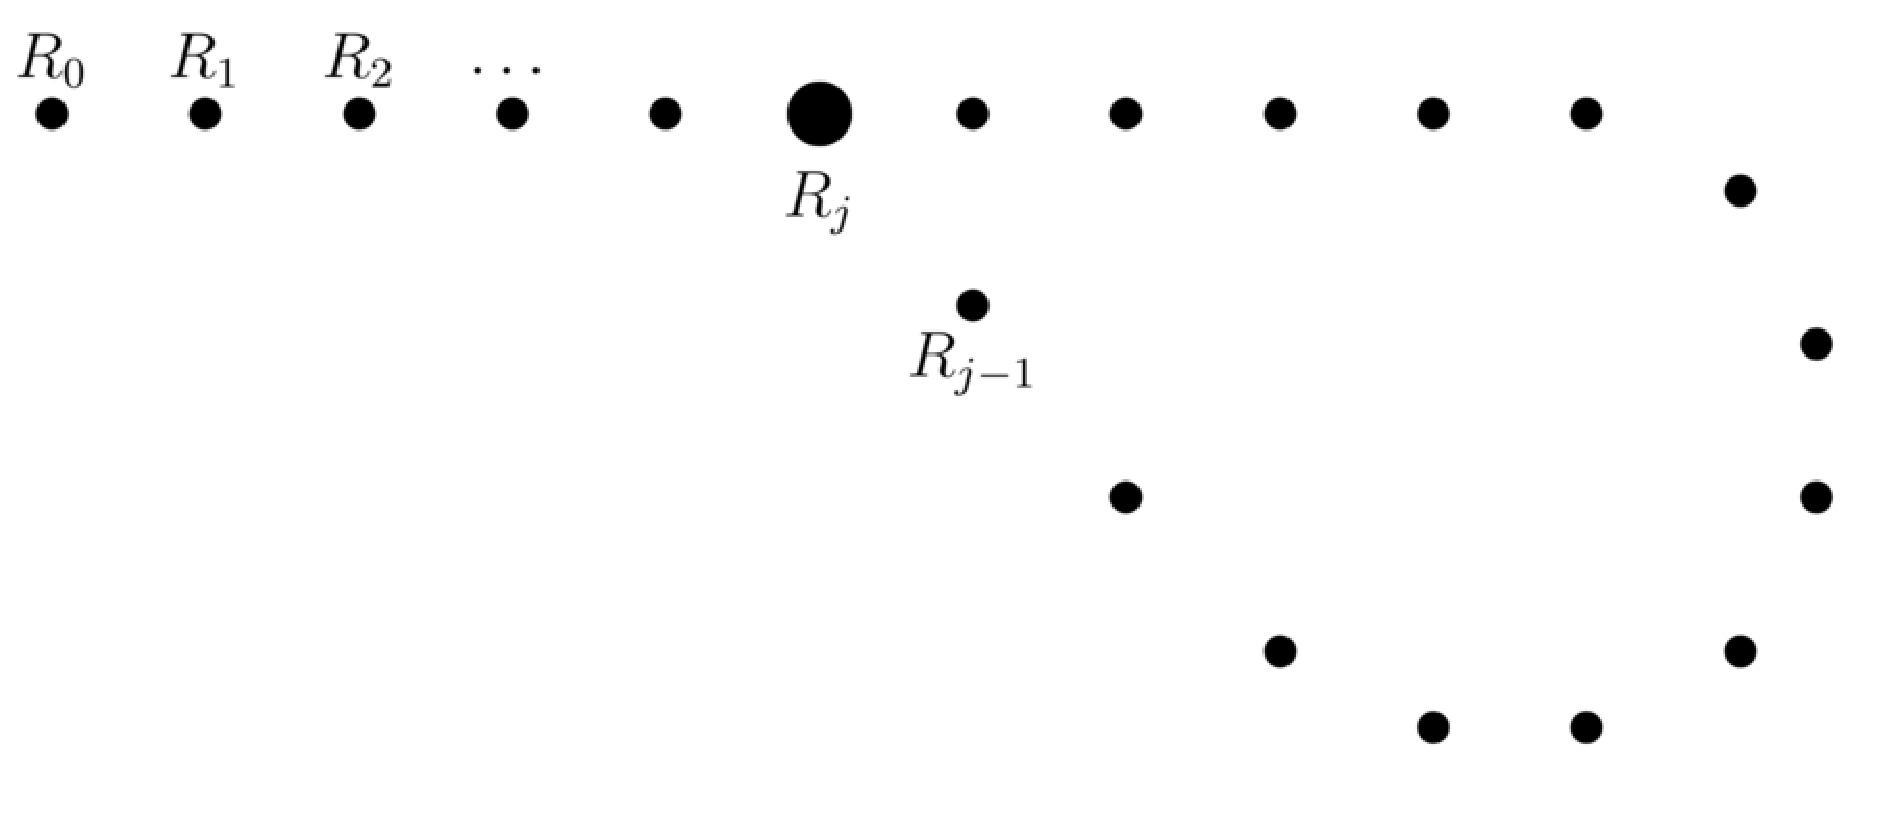
\includegraphics[scale=0.4, bb=0 0 888 376]{figuras/rho.eps}
% 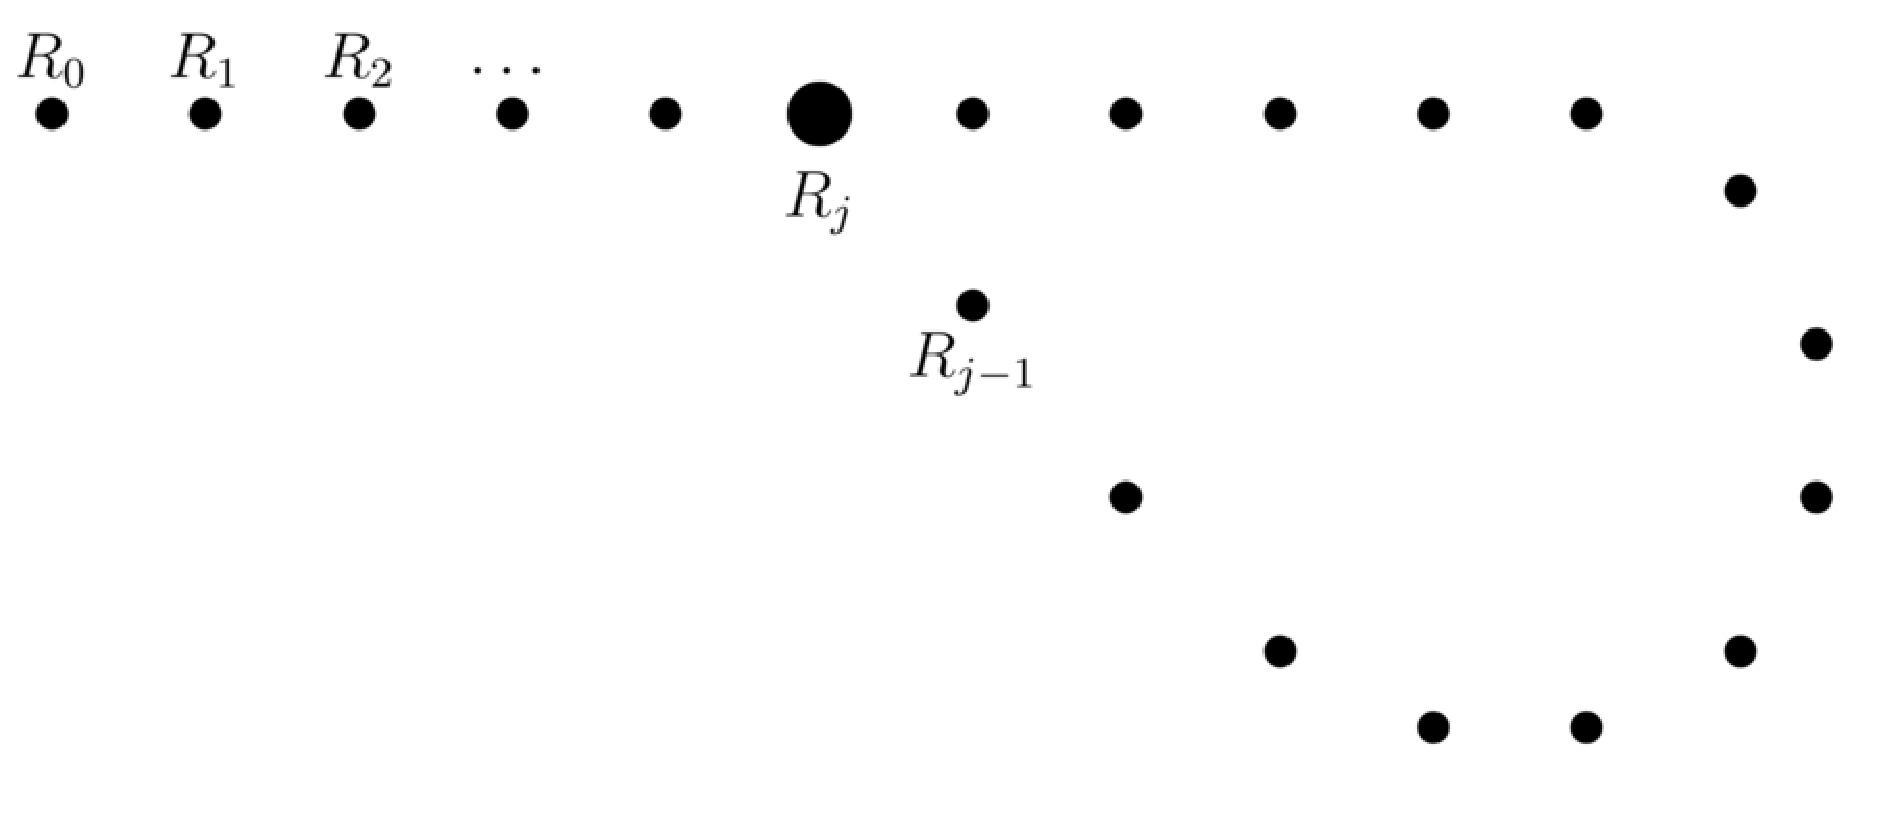
\includegraphics[scale=0.2, bb=0 0 1776 150]{figuras/rho.eps}
\caption{Diagrama da sequência produzida pelo algoritmo Pollard-Rho}
\label{fig:rho}
\end{figure}
